\section{Theoretischer Hintergrund}
Eine Pelton-Turbine, wie in \autoref{fig:Peltonturbine} zu sehen, gehört zu den Gleichdruckpumpen, d.h. direkt vor und hinter der Turbine herrschen der gleiche Druckverhältnisse.\\
Für den im Folgenden betrachteten Versuch handelt sich hierbei um Umgebungsdruck.\\
\begin{figure}[H]
    \centering
    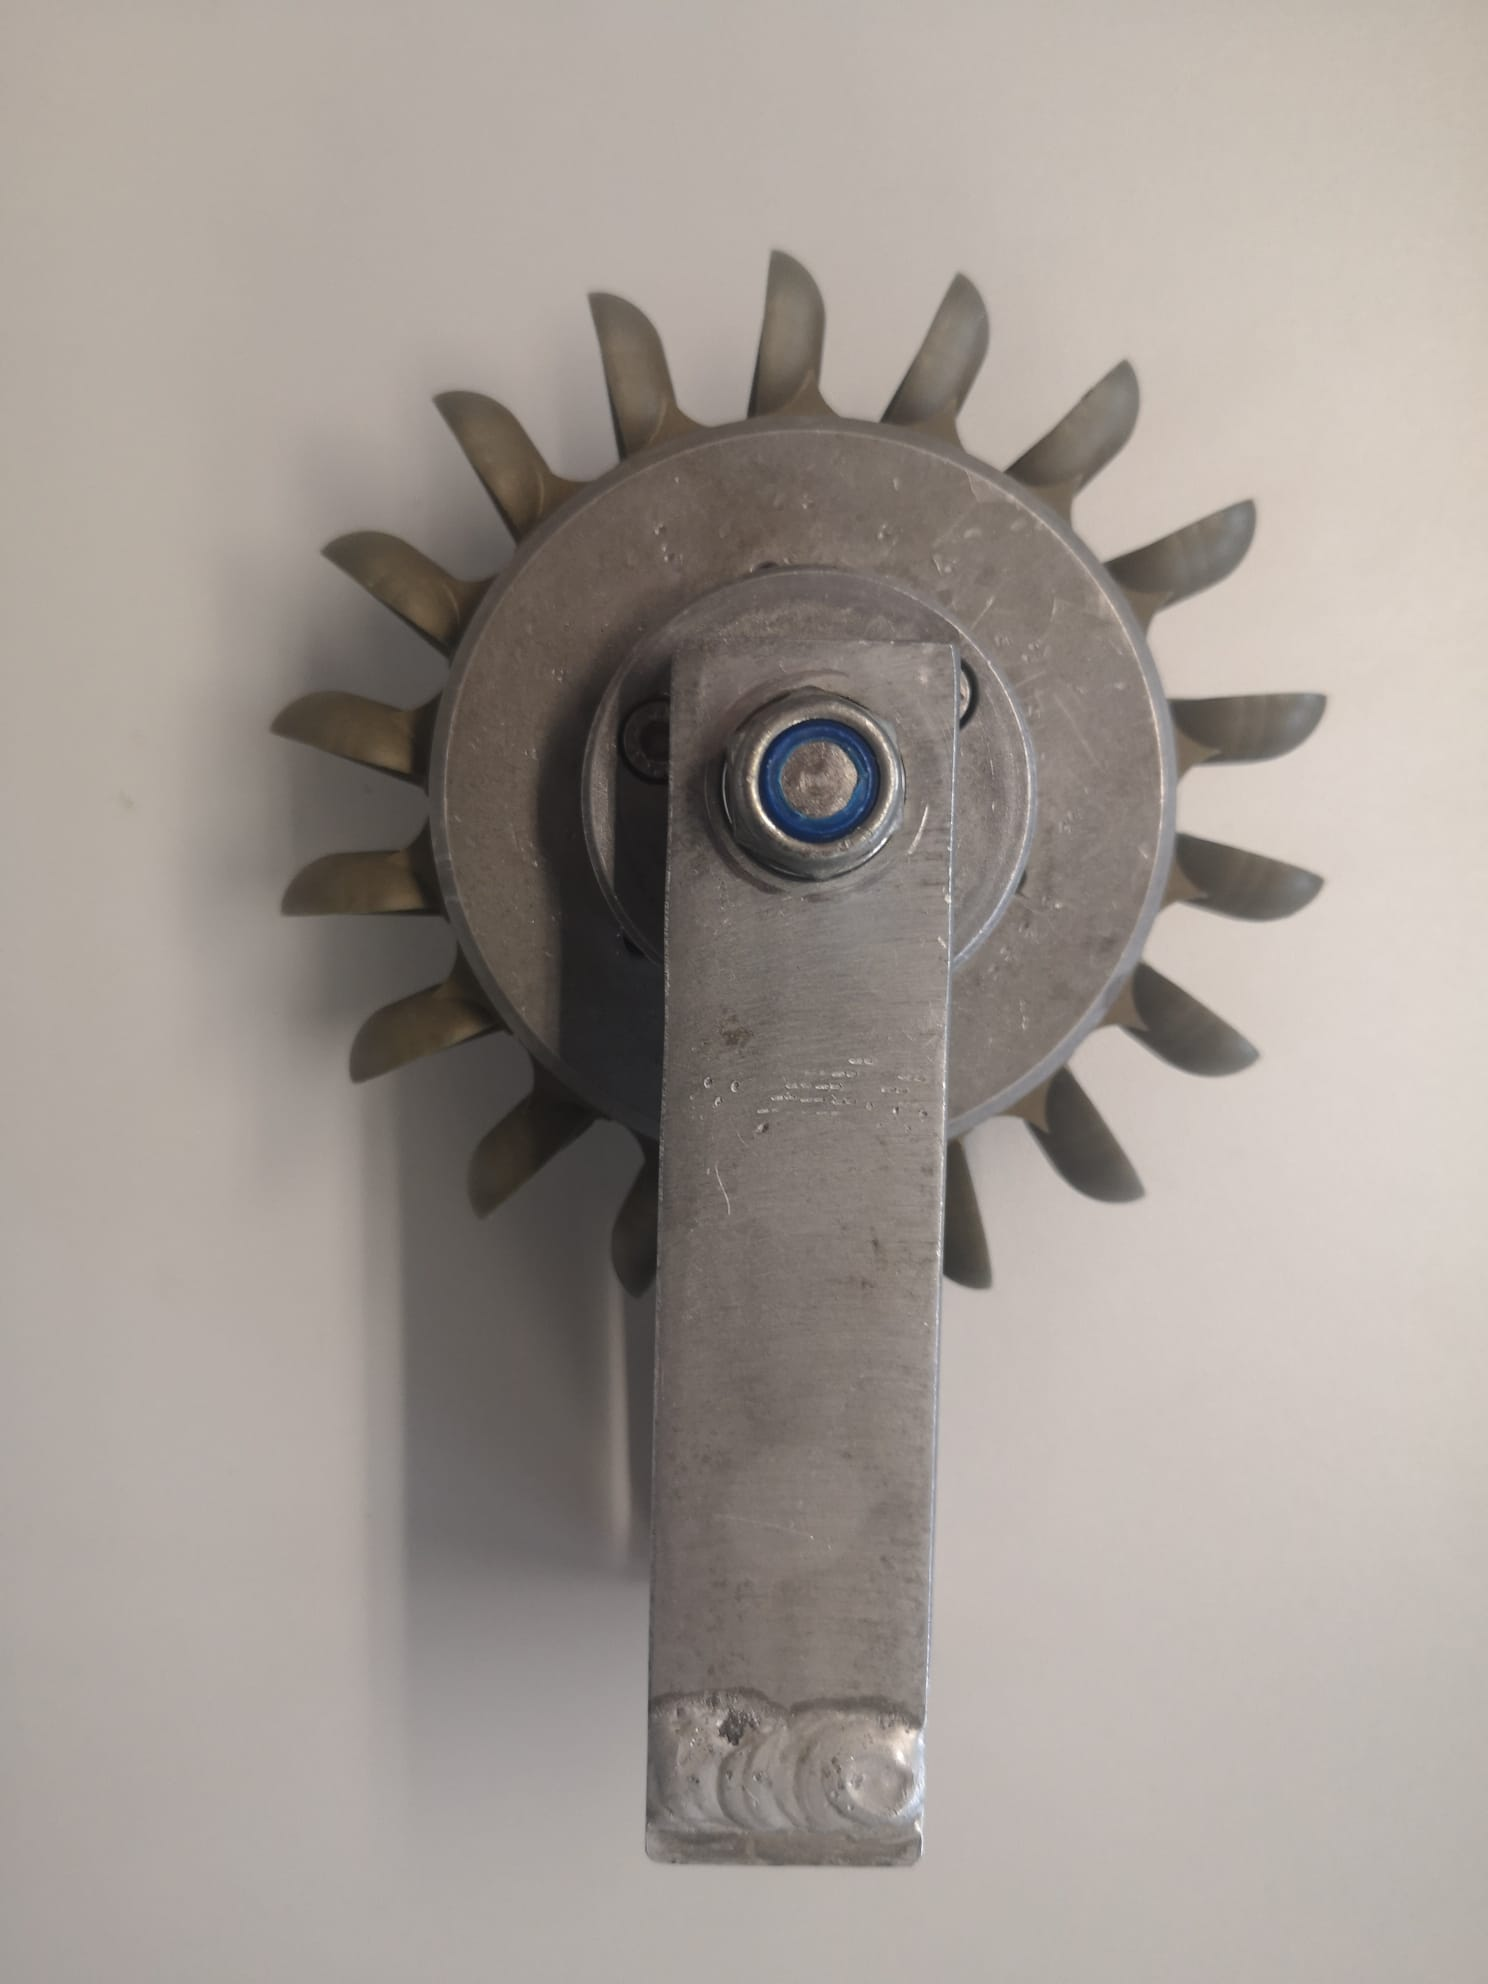
\includegraphics[width=0.5\textwidth]{Abbildungen/Peltonturbine.jpeg}
    \caption{Peltonturbine}
    \label{fig:Peltonturbine}
\end{figure}

Aufgrund dessen, dass die Pelton-Turbine bei großen Förder- bzw. Fallhöhen und geringen Volumenströmen sehr effizient arbeitet,
eignet sich diese Art Turbine ideal für die Energiegewinnung durch Wasserkraft.
Die physikalische Grundlage hierfür liegt der kinetischen Energie des durchströmenden Wassers.
Für die Berechnung der hydraulische Leistung dient hierbei die \autoref{eq:hydraulische_Leistung}.

\begin{equation}
    P_{Hyd.} = \rho \cdot g \cdot Q \cdot H
    \label{eq:hydraulische_Leistung}
  \end{equation}

Für die Berechnung sind die Verluste innerhalb der vorgeschalteten hydraulischen Anlage von Relevanz,
hierfür ist die Berechnung der Druckhöhenverluste mittels \autoref{eq:Druckhöhenverluste} notwendig.
Hierbei werden sowohl die Rohreigenschaften als auch die Einflüsse aller Einbauten berücksichtigt.
\begin{equation}
    H_{V} = \frac{\lambda \cdot l \cdot v_{r}^2}{2 \cdot g \cdot d} + \sum_{i=0}^{i} \frac{\zeta_{i} \cdot v^2}{2 \cdot g}
    \label{eq:Druckhöhenverluste}
\end{equation}

Darüber hinaus sind auch die mechanischen Eigenschaften der Pelton-Turbine von Bedeutung.
Die hierfür zentrale mechanische Leistung berechnet sich entsprechend \autoref{eq:MechanischeLeistung}.

\begin{equation}
	P_{Mech.}= M \cdot 2 \cdot \pi \cdot n
\label{eq:MechanischeLeistung}
\end{equation}

Hierbei lassen sich über die Einstellung der Düse und weiterer Komponenten unter anderem die Strahlgeschwindigkeit
und infolgedessen auch die Umfangsgeschwindigkeit sowie Drehzahl ändern.\\
Die Zusammenhänge dieser Größen sind in \autoref{eq:austrittsgeschwindigkeit},\autoref{eq:umlaufgeschwindigkeit} und \autoref{eq:n-optimal} dargestellt.

\begin{equation}
    c_{0}=\frac{4 \cdot Q}{\pi \cdot D_{D}^2}
      \label{eq:austrittsgeschwindigkeit}
    \end{equation}

  \begin{equation}
    u_{opt} = \frac{c_{0}}{2}=\pi \cdot u_{opt} \cdot d_{2}
    \label{eq:umlaufgeschwindigkeit}
  \end{equation}
    
    \begin{equation}
     n_{opt}=\frac{c_{0}}{2 \cdot \pi \cdot d_{2}}=\frac{2 \cdot Q}{d_{2} \cdot \pi^2  \cdot D_{D}^2}
    \label{eq:n-optimal}
    \end{equation}
